
\section{Data sources and adjustments}
\label{sec:dataprep}
Data presented here are from several different data sources, covering different time periods. These data originate in different age-period-cohort (APC) bins, and some are derived using indirect methods or projection methods. The full list of sources is outlined in Tab.~\ref{app:sources}. Fig.~\ref{fig:histbins} depicts the discrete Lexis bins of input data for the historical period before 1891. This appendix describes all steps taken to bring data into a standard format suitable for this study, and sections follow the order of the data processing steps undertaken. The data format required to build the figures in this manuscript consists in birth counts tabulated by single year of occurrence and mother cohort, the period-cohort (PC) Lexis shape (also denoted as `VV' in HFD documents). Input data cover the years 1736 until 2016, with an oldest mother cohort of 1687. We complete the fertility of incomplete cohorts through 2016 up to age 55, bringing the latest year of occurrence to 2071.

\begin{table}[ht]
\begin{tabular}{lllllc}
From & To & Data & Bins & Use & Source \\ \hline
1736 & 1750 & birth counts & totals only & constraint & SCB \\
1751 & 1755 & life tables & single ages 0-110 & reverse survival & HMD \\
1751 & each & population census & abridged ages & base for retrojection & HMD \\
1751 & 1774 & ASFR & single-age, 5-year & \makecell{infer births 1751-1774 \&\\ derive retrojection standard} & HFC \\
1751 & 1774 & population exposures & single-age and year & infer births & HMD \\
1751 & 1774 & birth counts & totals only & constraint & HMD \\
1775 & 1890 & birth counts & abridged ages & constraint & SGF \\
1891 & 2016 & birth counts & single ages & as-is & HFD \\
1966 & 2016 & ASFR & single ages & rate projection & HFD \\
2017 & 2071 & Population projections & single ages & infer completed fertility & SCB
\end{tabular}
\caption{Data sources}
\label{app:sources}
\end{table}

\begin{figure}[ht!]
\begin{center}
\includegraphics[scale=.65]{Figures/HistoricalDimensions.pdf}
\vspace{-2em}
\caption{Lexis diagram depiction of fertility data sources and discrete Lexis bins for the period 1736-1890. Total counts are used as constraints for years 1736-1750, denoted with red boxes at age 0. The yellow box from 1736 to 1750 denotes the Lexis region over which birth counts are reconstructed using indirect techniques. The blue boxes from 1775 to 1890 indicate various age-period bins of birth counts. Light blue indicates lower and upper open age groups. Dark blue boxes in ages 14-19 from 1861-1890 indicate single year age-period bins. The HFD provides single-year period-cohort bins for birth counts starting in 1891 (gray).}
\label{fig:histbins}
\end{center}
\end{figure}

\FloatBarrier
\subsection{Years 1736 - 1750}
\label{app:retroject}
Estimating birth counts by single year of age for the 15 year period from 1736 to 1750 requires several steps of data processing and some strong assumptions. First, we reverse-survive  females observed in the 1751 mid-year population census of Sweden, as extracted from the \citet{HMD} input database. Since this is a July 1 census, we take it as an acceptable proxy for exposure. The census originates in abridged ages $[0,1,3,5,10,15~...~90+]$. Examination of five year age groups suggests a underlying pattern age heaping, and for this reason we first smooth them using the so-called United Nations method \citep[see ][]{carrier1959reduction} as implemented in the \texttt{DemoTools} \texttt{R} package \citep{demotools}. We then graduate to single ages using the Sprague method \citep{sprague1880explanation,Shryock1973} as implemented in the \texttt{DemoTools} \texttt{R} package. This population is now the basis population to be reverse-survived through each single year until 1736, where we only make use of the fertile ages.

To reverse-survive, we use a standard survival curve defined as the age-specific arithmetic mean of the five single-age life table survival functions for the years 1751-1755 \citep{HMD}. The mid-year population count at age $x$, $n$ years before the 1751 census $P(x,1751-n)$ is estimated as:
		\begin{equation}
\label{eq:Pxhat}
P(x,1751-n) = P(x+n,1751) * \frac{\ell(x)}{\ell(x+n)} \tc
\end{equation}
where $\ell(x)$ is the standard survival function described.

The next step is to derive a standard age-specific fertility rate (ASFR) curve, $F(x)$. ASFR for the years 1751-1775 is given by the \citet{HFC} in single ages and 5-year bins. If we rescale $F(x)$ in each 5-year period to sum to 1, one sees that there was very little shifting or shape changes in the period 1751-1774: each unity-scaled $F(x)$ curve is for practical purposes equivalent. We therefore take the standard fertility rate curve, $F^\star(x)$ to be their age-specific arithmetic mean, and we assume that it is valid for the year-range 1736 until 1750.

A first pass of unscaled birth counts at age $x$, $t$ years before 1751 is taken as the product of estimated exposure and $F^\star(x)$.
\begin{equation}
\widehat{B}^\star(x,1751-n) = P(x,1751-n) \cdot F^\star(x)
\end{equation}

The first pass of birth estimates implies a total fertility rate of 1 in each year. Total births in each of these years $B(1751-n)$ is known \citep[][Tab.~27 \& Tab.~28]{sweden1969historisk}, so we derive our final estimate of age specific births, $\widehat{B}(x,1751-n)$ as:
		
		\begin{equation}
\widehat{B}(x,1751-n) = \widehat{B}^\star(x,1751-n) \cdot \frac{B(1751-n)}{\sum _{x=12}^{50}\widehat{B}^\star(x,1751-n) }
\end{equation}

At this stage of processing, birth count estimates for the years 1736-1750 are given in single ages (AP Lexis squares). Further adjustments are carried out in common with later periods and described in the following sections.

\subsection{Years 1751 - 1774}
\label{sec:hfc}
Estimating birth counts in single years and by single year of age for the 24 year period from 1751 to 1774 follows a similar logic, but it requires no retrojection. The \citet{HFC} provides ASFR in single ages\footnote{This data was graduated by the HFC from 5$\times$5 Lexis cells according to the HFC methods protocol \citep{grigorieva2015methods}.} in 5-year bins. The HMD provides exposure estimates $P(x,t)$ in single ages and years over this same period. A first-pass estimate of birth counts, $\widehat{B}(x,t)$ is given by:
		
		\begin{equation}
\widehat{B}(x,t) = P(x,t) \cdot F(x,t') \tc
				\end{equation}
				
				where $t'$ denotes the 5-year bin in which $t$ happens to fall. Year bins in the data are 5-years wide, and shifted up by 1, ergo 1751-1755, 1756-1760, and so forth. Following the convention of indexing to the lower bound, $t'$ is defined as:
				\begin{equation}
				t' = 5\floor{t/5}+1
				\end{equation}

Births by single year of mothers' age are then rescaled to sum to the annual totals reported in the HMD:
		\begin{equation}
		B(x,t) = \widehat{B}(x,t) * \frac{B(t)}{\sum _{x=12}^{50}\widehat{B}^(x,t)}
		\end{equation}
		
		At this stage of processing, birth count estimates for the years 1751-1774 are given in single ages (AP Lexis squares). Further adjustments are carried out in common with later periods and described in the following sections.
		
		\subsection{Years 1775 - 1890}
		\label{sec:sgf}
		Birth counts for the 116 year period from 1775 to 1890 are available from \citet{sgf1907}. These data are age-period classified, and given in a mixture of age classes, with a
		predominance 5-year age classes (especially for ages 20-50), but also sometimes
		single ages (especially for ages 15-19), and time-varying top and bottom open
		ages. We standardize these data in a few simple steps.
		
		First, births of unknown maternal age were redistributed proportionally to the distribution of births of known maternal age. Second, counts are graduated to single ages using the graduation method proposed by \citet{rizzi2015efficient} and implemented in \texttt{R} in the package \texttt{ungroup} \citep{ungroup}. 
		
		\subsection{Years 1736 - 1890}
		\label{sec:histadj}
		At this stage of processing all birth counts for years 1736 until 1890 are in single age-period (AP) bins, and datasets covering the three periods are merged into a common dataset. Two further adjustments are performed, the first to move AP into PC bins. The second adjustment compensates for the smoothness of graduation methods so as to preserve the expected relationship between a cohort's size its total offspring size.

\subsubsection{Adjustment to PC bins}
\label{sec:split}
Counts were shifted from AP Lexis bins into PC bins assuming that half of the births in each single age $x$ bin go to the lower triangle of age $x+1$ and half to the upper triangle of the age-reached-during-the-year (PC) parallelogram at age $x$, as diagrammed in Fig.~\ref{fig:AP2PC}. This simple assumption could be made more sensitive, but it would have no noticeable impact on our visualization. At this point data are in a common format with the HFD data for the years 1891-2016, and these are merged into a single dataset.

\begin{figure}[ht!]
\centering
\begin{subfigure}{.3\textwidth}
\centering
\includegraphics[scale=.5]{Figures/App_split1.pdf}
\caption{AP square bins}
\label{fig:app1}
\end{subfigure}%
		\begin{subfigure}{.3\textwidth}
\centering
\includegraphics[scale=.5]{Figures/App_split2.pdf}
\caption{Split evenly to triangles}
\label{fig:app2}
\end{subfigure}
\begin{subfigure}{.3\textwidth}
\centering
\includegraphics[scale=.5]{Figures/App_split3.pdf}
\caption{Regroup to PC bins}
\label{fig:app3}
\end{subfigure}
\caption{The count regrouping procedure for years 1736 to 1890. Data are graduated to single ages (Fig.~\ref{fig:app1}), then split in half (Fig.~\ref{fig:app2}) and regrouped to period-cohort (PC) bins (Fig.~\ref{fig:app3}).}
\label{fig:AP2PC}
\end{figure}

\FloatBarrier
\subsubsection{Cohort size adjustment}
\label{sec:cohadj}
At this stage of processing we have a harmonized dataset comprising a single series from 1736 until 2016 in consistent single-year PC bins. As such, one could produce the two time series represented in Fig.~\ref{fig:foldout}, albeit with a subtle artifact visible in Fig.~\ref{fig:toosmooth}. In area \textbf{A} of this figure, birth counts in age bins have been graduated using the previously mentioned pclm method, which has the usually-desired artifact of smoothness. For the affected range of years, mother cohorts are identified via the identity $C = P - A - 1$ .\footnote{One subtracts 1 because data are in period-cohort bins.} Since age patterns of counts are smooth, these sum in Lexis diagonals to a smooth time series of cohort total offspring, as seen in the profile of area \textbf{B} of the same figure. Area \textbf{C} of this figure delimits years 1875 until 1971, where both cohort and matched offspring sizes are directly observed,\footnote{We estimate that the fertility of the 1971 cohort was over 99\% complete as of 2016.} and where fluctuations would appear to co-vary quite strongly. For the sake of a more sensible count graduation and for reasons of aesthetic continuity, we have opted to adjust the counts in area \textbf{B} to carry the pattern of fluctuation observed over cohort size from 1736 to 1890.

\begin{figure}[ht!]
\centering
\includegraphics[scale=.6]{Figures/App_preAdjustment.pdf}
\caption{In reference years $\ge$ 1891 both births by year and cohort offspring are directly observed in single year bins, which means that the structural echo between total birth cohort and offspring size is preserved for reference years $\ge$ 1876  (\textbf{C}). Total per annum births in years $\le$ 1890 (\textbf{A}) are presumed accurate, and so first differences of these are observed. Offspring from cohorts born in years $\le$ 1876 (\textbf{B}) were partially (1836--1876) or entirely ($<$ 1836) born in years $\le$ 1890, implying a smooth redistribution over single years of mother cohorts. We wish to adjust the births in \textbf{B} to recuperate the kind of structural echo in \textbf{C}.}
\label{fig:toosmooth}
\end{figure}

This adjustment works by extracting the fluctuation pattern from \textbf{A} and transferring it to \textbf{B}. We do this by first smoothing the annual time series of total cohort size $B(t)$ according to some smoothness parameter, $\lambda$.\footnote{For the present case we've used a loess smoother, using the \texttt{R} function \texttt{loess()} with smoothing parameter $\lambda =$ \texttt{span}. It would be straightforward to swap this smoothing method out with a different one.} The ratio of $B(t)$ to the smoothed birth series $B(t)^s$ defines the multiplicative adjustment factor, $adj(t) = B(t)/B(t)^s$. Total offspring size $\mathbb{B}(c)$ is then adjusted as $\mathbb{B}(c)' = adj(t)*\mathbb{B}(c), \mathrm{~for~} c = t$. Counts in single ages are then rescaled to sum to the original totals in 5-year age groups, and counts for years $>$ 1890 are unaffected. The smoothing parameter is selected such that the linear relationship in fractional first differences $rd(B(t)) = \frac{B(t+1)-B(t)}{B(t)}$ between the annual birth series and adjusted offspring series $rd(\mathbb{B}(c)')$ for years 1736-1876 matches that for the reference years 1877-1971 as closely as possible. Specifically, we select $\lambda$ so as to minimize the sum of the difference in slopes and residual standard deviations for the periods before and after 1891. Further clarifications about this adjustment, and code for diagnostic plots can be found in the annotated code repository. The end effect is to adjust the series to look like Fig.~\ref{fig:better}.
					
					\begin{figure}[ht!]
					\centering
					\includegraphics[scale=.6]{Figures/App_postAdjustment.pdf}
					\caption{The adjusted birth series. Annual total births $B(t)$ on top axis and annual total offspring $\mathbb{B}(c)$ on bottom axis, with adjusted offspring counts $\mathbb{B}(c)'$ outlined.}
\label{fig:better}
\end{figure}


We adjusted in this way for the sake of a more nuanced time series of total offspring, but this approach may be used to good effect in graduating age-structured counts (births, deaths, populations) whenever time series are long enough to permit information on birth cohort size to propagate through the Lexis surface. These aspects are visible to some degree in the shaded polygons of Fig.~\ref{fig:foldout} in years $<$ 1891.

\FloatBarrier
\subsection{Projected birth counts}
\label{sec:proj}
Offspring counts by year of occurrence, $B(c,t)$ are only fully observed for years $\le$ 1961. To complete the offspring reflection through the final reference year 2016, we have opted to project birth counts for cohorts whose fertility careers are incomplete (1962-2016). This is done by combining a projection of cohort fertility rates using the method proposed by \citet{de1985time} with Sweden's official projection of population denominators \citep{SCBpop, SCBproj} to derive the implied birth counts by single year of age and time. The method used is parsimonious, and it performed very well in a comprehensive assessment of fertility forecast methods \citep{bohk2018forecast}. This outstanding forecast performance can partly be explained with the model's ability to capture changing levels of fertility across ages and cohorts with two integrated ARIMA time series processes. In our application for Swedish birth counts the model of de Beer is fitted to observed fertility rates at ages 12 through 55 in calendar years 1967 to 2016 in order to complete the fertility for cohorts 1962 through 2004 and fully forecast the fertility of cohorts born 2005 through 2016.

\begin{figure}[ht!]
\begin{center}
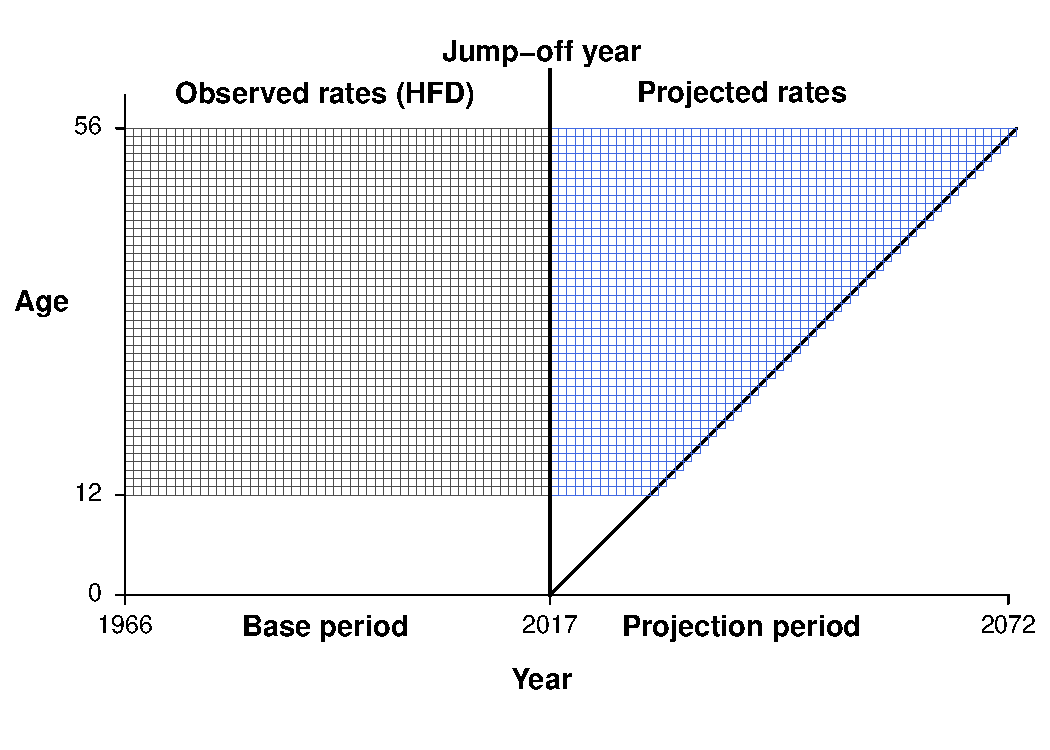
\includegraphics[scale=.65]{Figures/ProjectionDiagram.pdf}
\caption{Diagram of the age and year-range of fertility rates used for model fitting and projection. We fit to 50 years of data (1966 until 2016), and project until the 2016 cohort (right bound of 2017) reaches age 55 in the year 2071 (right bound of 2072). The diagonal line delimits the data range after splitting to period-cohort bins.}
\label{fig:projdiag}
\end{center}
\end{figure}

Projected rates are then multiplied with SCB projected female population counts to derive implied births by age of mother. The projected birth counts are in single year age-period bins. These are then split to vertical parallelograms using the simple method described in Appendix~\ref{sec:split}. The upward-slanting diagonal line in Fig.~\ref{fig:projdiag} marks the edge of the 2016 cohort fertility.

%Light documentation to follow here, as well as an update of Fig.~\ref{fig:better}.

\FloatBarrier
\subsection{Meandering baseline}
\label{sec:baseline}
A peculiar feature of Fig.~\ref{fig:foldout} is the meandering baseline, which replaces the standard straight-line $x$-axis. The baseline is derived from the crude cohort replacement rate $\mathbb{R}(c)$, defined as $\mathbb{R}(c) = \mathbb{B}(c=r) / B(t=r)$. This measure is not a replacement for the classic measure of net reproduction $R_0$, which differs in a few key ways: i) crude replacement is not sex-specific (our birth series is composed of boy and girl births combined), whereas $R_0$ is typically defined for females only. ii) while births arise from fertility rates over the life course, the number of potential mothers over the life course is not a mere function of mortality, but of migration as well, and the Swedish birth series will have been affected by heavy out-migration from 1850 until the Second World War, and some in-migration in more recent decades. Cohort $R_0$ is purged of population structure such as this (except to the extent that subgroups have differential vital rates), whereas $\mathbb{R}(c)$ is not, and for this reason we call it \emph{crude}.

The series of $\mathbb{R}(c)$ is rather smooth without further treatment, save for 11 periodic breaks between 1970 and 1840, a period of rupture between 1865 and 1880, and another set of at least four breaks since the great depression in the 1930s. Rather than preserve these ruptures, we opt to smooth them out and instead capture long term trends in $\mathbb{R}(c)$ in the baseline, as seen in Fig.~\ref{fig:meander}. Keeping the baseline meander smooth minimizes the visual penalty in assessing the variation in $\mathbb{B}(c)$ or $B(t)$ separately, and it enhances our ability to see the long term pattern. Specifically, we use use the \texttt{smooth.spline} from the \texttt{stats} \texttt{R} package, to smooth the $ln(\mathbb{R}(r))$ with smoothing parameter $\lambda = 0.00001$. The baseline that appears in Fig.~\ref{fig:refl} is the smooth prediction multiplied by 100,000.

\begin{figure}[ht!]
\centering
\includegraphics[scale=.6]{Figures/Meander.pdf}
\caption{The time series of crude cohort replacement, $\mathbb{R}(c)$, and its smooth pattern (blue line) on which the Fig.~\ref{fig:foldout} meandering baseline is based.}
\label{fig:meander}
\end{figure}



